\documentclass[11pt,a4paper]{jsarticle}
%
\usepackage[dvipdfmx]{graphicx}
%
\usepackage{comment}
\usepackage{tipa}
\usepackage{natbib}
\usepackage{url}
\usepackage{gb4e}
\usepackage{float}
\usepackage{ascmac}

\bibpunct[: ]{(}{)}{,}{a}{ }{,}
%
\setlength{\textwidth}{\fullwidth}
\setlength{\textheight}{39\baselineskip}
\addtolength{\textheight}{\topskip}
\setlength{\voffset}{-0.5in}
\setlength{\headsep}{0.3in}
\setlength{\oddsidemargin}{0pt}
\setlength{\evensidemargin}{0pt}
\newcounter{tempcnt}
\newcommand{\exn}[1]{%
\setcounter{tempcnt}{\value{exx}}%
\addtocounter{tempcnt}{#1}%
\arabic{tempcnt}}
%
\title{\fontsize{16pt}{0pt}\selectfont ソロモン諸島のピジン(Pijin)語における従属節標識について}
\author{栗田健太郎}
\date{2019年12月4日}

\markright{\footnotesize \sf 言語学卒論演習(2019-12-4)栗田健太郎}

\begin{document}
\maketitle
\section{Pijin語について}
\paragraph{Pijin語}\footnote{現地では単に\textit{pijin}と呼び、英語の文献では種類としてのピジン語を``pidgin language'', ソロモン諸島に存在する(本発表で扱う)言語を``Pijin''と表記することが多いようである。この資料においては前者をピジン言語、後者をPijin語と表記する。}\footnote{グロスで用いる略号は基本的に\cite{prepositions}に従ったが、いくつかの必要な略号は補った: 1/2/3=1st/2nd/3rd person, SG=singular, DU=dual, PL=plural, INC=include, EXC=exclude, DEIC=deictic, PM=predicate marker, FUT=future, PERF=perfective, NEG=negative, DAT=dative, TOP=topic} ソロモン諸島の事実上の共通語。公用語の地位は与えられていない話し言葉

\subsection{歴史と言語状況}
\cite{phonology}
\paragraph{歴史}
\begin{itemize}
  \item Melanesian Pidgins(Tok Pisin[PNG], Bislama[Vanuatu], \textbf{Pijin}[Solomon Islands])の1つ
  \item 豪クイーンズランドでのプランテーションに従事していた労働者がソロモン諸島へ持ち帰る
  \item その後ソロモン諸島がイギリスに併合される(1893)$\rightarrow$イギリス人や他の島民と話す手段に
  \item ソロモン諸島国内でもプランテーション開始(1920頃)$\rightarrow$様々な島から来た労働者へ広まる
  \item 1960年頃から首都ホニアラでの主要言語に
\end{itemize}

\paragraph{ソロモン諸島の共通語として}
\begin{itemize}
  \item ソロモン諸島は言語的に多様、首都ホニアラでは64の言語が話されているという
  \item 1つの言語を話す集団=wantok
  \item wantokの間ではその言語を話し、wantokの異なる者同士が話すときにPijinを用いる
  \item 都市化や教育の発展により、Pijinを用いる頻度は劇的に増加
  \item 田舎部では依然第二言語であるが、都市部ではPijinを母語として育った人も増えている
\end{itemize}
\subsection{Pijin語と他言語}
\paragraph{Pijin語と英語} 語彙供給源は英語。イギリスに支配されていた歴史的背景もあり、一帯の中で最も英語に近いと言われる

\begin{quotation}
  英語のPijin語への影響は直ちに明らかである。Pijin語の辞書\citep{yumi}を見れば、そこに定義されている語の95\%が英語に由来することが分かる。地元のメラネシア語の影響も同様に明白で、広く行き渡っているが、一般的にはより捉えがたい。一般的に、英語の貢献は形式と主な意味のレベルでより大きく、一方、現地の言語の貢献は文法と派生的な意味のレベルでより大きくなっている。\citep{malaitan}\footnote{訳は発表者。原文: The influence of English on Pijin is immediately obvious. A scan through the Pijin dictionary (Simons and Young 1978) shows that 95 per cent of the words defined there have borrowed their form from English. However, the influence of local Melanesian languages is evident as well, equally as pervasive but generally more subtle. As a general rule the contribution of English has been more at the level of form and primary meaning, while the contribution of the local languages has been more at the level of grammar and extended meanings.}
\end{quotation}
\cite{nativization}
\begin{itemize}
  \item 都市化や母語化に伴い、都市部のPijin語は変化している
  \item 都市の話者の多くはPijin語と英語双方の知識があるため、Pijin語も徐々に英語化?
  \item 言語的なバリエーションは大きく、ラジオなどで用いられる英語に近いPijin語は話者の一部にとって英語でもPijin語でもない
  \begin{itemize}
    \item ``\textit{Diskaen Pijin ia hemi rabis tumas}'' (このPijin語は最悪だ)
  \end{itemize}
\end{itemize}

この論文では都会のPijin語において、英語由来の単語が増えていること、英語にはない文法事項が消滅してきていること、逆に英語の文法事項\footnote{形態的レベルでの最も明白な変化として、\cite{nativization}は英語の複数マーカーの借用について述べている。
\begin{exe}
  \exi{(i)} Olketa pleses ia. \hspace{0.6in}``These places."
  \exi{(ii)} Olketa ples ia.
  \exi{(iii)} Pleses ia.
\end{exe}
Pijin語で複数を表現するには、本来は名詞の屈折ではなく、三人称複数の代名詞である\textit{olketa}を名詞の前に付けて(ii)のように示していた(ただし義務的ではない)が、最近はその際に(i)のような複数接尾辞(\textit{-s},\textit{-es})が名詞に付くことがあるという。
この論文では(iii)のように名詞接尾辞だけで複数を表す用例はないと書かれているが、私の観察では、\textit{olketa}無しで複数接尾辞が登場する例もたくさん見つかった。ただし、いずれも非常に英語的な表現の中や近くに見つかり、話者はPijin語本来の表現と区別しているように感じる。\cite{manguru}には多くの例が見られるが、書き言葉である聖書からは完全に排除されている。
\begin{exe}
  \exi{(iv)}
  \gll Mifala traim fo duim samfala \underline{criterias} fo chusim \underline{which} \underline{areas} an \underline{sites}.\\
  1PL.EXC try to do some criteria-PL for choose which area-PL and site-PL\\
  \glt `We tried applying various criterias for choosing areas and sites.'(\cite{manguru}, 1分26秒)
\end{exe}
\textit{which}も\textit{criteria}もPijin語の辞書には登場しない単語である。この話者は他の部分では\textit{olketa(ota)}+名詞の形式も使っている。
}がPijin語の中に入ってきていることについて述べている。発表者の滞在中にも、疑問詞\textit{wanem}が\textit{what}に置き換わっている、主語の代名詞による繰り返しが消えている(あるいは、主語の数に関わらず常に単数形の代名詞\textit{hem}が用いられる)など、その進行ははっきりと感じた。

この論文は、その理由は脱クレオール化ではなく、文法変化はあくまでPijin語自体の枠組みの中で起こっているとし、見かけ上の英語化は英語とPijin語とのコードスイッチングによるものであると結論づけている。

今回の従属節標識についても、\textit{dat}、\textit{fo}いずれも英語からの翻訳文体に多く見られ、英語からの影響があることは十分推測できるが、しかしいずれも英語の使い方と完全に同じわけではない。よって、私は見かけ上の英語化は脱クレオール化(英語との同化)ではなく現代のコードスイッチングがもたらしたものであるという\cite{nativization}の主張に賛成する。

\section{Pijin語の従属節標識について}
Pijin語で手に入るまとまった書き言葉として、事前に新約聖書 \footnote{Bible.is \url{https://live.bible.is/bible/PISWBT/}に掲載されている本文を使用。テキストの提供者としてBible Society of the South Pacific, 翻訳者としてWycliffe Bible Translatorsがクレジットされている}をコーパス分析した。その結果、本来別の意味を持っている2つの単語が従属節標識のように使われていることが分かった: dat, fo。

調査はホニアラ市内で高校生から60代までの9人の話者を対象に行われ、全員がホニアラに10年以上住んでいるが、出身がホニアラの人は3人だけで、Pijinが母語だという人は1人だった。全員が学校教育を受けていて、Pijin語と英語双方の知識を持っていた。

これら2つの単語の意味を尋ねたところ、多くの場合は従来持っていた意味を説明されることが多かったため、調査では、従属節標識としてこれらの語が使われている例文をこちらから示し、この文が自然か、文章全体で不自然な部分があるかどうか尋ねた。その上で別の言い方は無いか、どのような状況でこう言うか等を尋ねた。終了後、調査の目的を伝えた上で、インフォーマント自身にdatやfoの使い方について聞いた。状況付きで例文を示してくれるインフォーマントもいた。

\subsection{dat}
\paragraph{従来の意味}
\begin{itemize}
  \item \cite{dictionary}: 形容詞接辞\textit{-fala}付きの形\textit{datfala}「その、それ」や名詞接辞\textit{-wan}付きの形\textit{datwan}「それ」が別々の項に建てられている
  \item インフォーマントに\textit{dat}の意味を尋ねたところ、まず「それ」を指す用法を答える人が多かった
  \item \textit{-fala}は現代のPijinでは無くても許容されることが多いようである。ただし\cite{dictionary}に変種としての記載は無い
\end{itemize}
\begin{exe}
\ex
\gll \underline{Datfala} tri ia, hem long lan blong mi ia.\\
\underline{that} tree DEIC 3SG at land of 1SG DEIC\\
\glt `That tree is on my land.'
\end{exe}
\paragraph{名詞節を形成する従属節標識として}
\begin{itemize}
  \item 聖書中には673の用例。\textit{save dat} know that: 168, \textit{somaot dat} show that 87, \textit{lukim dat} seems that: 72...
  \item 英語のthat節と同様に、名詞的従属節を作る標識として利用されている
\end{itemize}
\begin{exe}
\ex
\gll An yufala save \underline{dat} olketa samting ya i hapen tru nao.\\
and 2PL know \underline{that} PL thing DEIC PM happen truly PERF\\
\glt `And you all know that the things really happened.' (1TH 3:4)
\end{exe}
\begin{itemize}
  \item Pijin語の辞書\cite{dictionary}や彼の文法概要\cite{syntax}、その他の入門書\cite{yumi}には記載がない
  \item Pijin語の教科書\cite{eric}にはごく簡単な説明と例文が示されていた(後述)
\end{itemize}
\subparagraph{調査}
(\exn{1}),(\exn{2})共に発表者が作った文である
\begin{exe}
\ex\label{dat1}
\gll Hemi talem \underline{dat} yu stap long hia.\\
3SG-PM tell \underline{that} 2SG be at here\\
\glt `He told that you are here.'
\ex\label{dat2}
\gll Mi no save \underline{dat} hem nao draev.\\
1SG NEG know \underline{that} 3SG TOP drive\\
\glt `I didn't know that he will drive.'
\end{exe}

結果、全てのインフォーマントからこの文は適格であると認められた。意味の違いについて尋ねたところ、2つの文は完全に同じだと答えた。50代のインフォーマント\footnote{ガダルカナル島東部のAola村の出身で、母語はLengo[オーストロネシア語族、南東ソロモン諸語]。ホニアラに来てPijinを覚えたのは30年以上前}は自分以上の年代では\textit{dat}単体での使用は違和感を感じるかもしれないと答え、次のような3通りの言い方なら許されただろうと述べた。\textit{bae}は未来を示すマーカーだがPijin語にはっきりとした時制はなく\citep{eric}、発表者の感覚では他の節や文中の出来事から見た相対的な未来を示したいときに用いられる。

\begin{exe}
\exi{(\exn{-1}$'$)} Hemi talem \underline{bae} yu stap long hia.
\exi{(\exn{-1}$''$)} Hemi talem \underline{dat} \underline{bae} yu stap long hia.
\exi{(\exn{-1}$'''$)} Hemi talem yu stap long hia.
\end{exe}

その後60代のインフォーマント\footnote{マライタ島南部出身、母語はBaelelea[南東ソロモン諸語]}に尋ねたが、彼女はこのような傾向を見せず、(\exn{-1})から(\exn{-1}$'''$)すべての文章が等しく正しいと答えた。

\cite{eric}\vspace{0.1in}
\begin{quote}
\begin{exe}
  \exi{3.} Mi talem hem dat Bili hem i stap long Kukum. \\
  `I told him that Billy lives in Kukum.'
\end{exe}\vspace{0.1in}
Some verbs in Pijin can take \underline{\texttt{dat*}} + SENTENCE as an object instead of a simple noun phrase.
\begin{screen}
NOTE: *There are many areas in the Solomons where \underline{\texttt{dat}} is not used: Speakers who don't use \underline{\texttt{dat}} will say that the two clauses with an intonation that suggests that they are two independent sentences, or use a word borrowed from a local language.
\end{screen}
\end{quote}
\begin{itemize}
  \item ラジオから録音した牧師の説話や読み上げてもらった際の録音を確認した
  \item (1)短い発話では、動詞に続いて間を置かずに話される (2)ゆっくりの発話では、文が続くことを示すために動詞の語尾が下降しない という特徴があるように思われる
  \footnote{通常の叙述文では文末の単語は下降する。

  \begin{quote}
    One common intonation pattern for declarative sentences starts at mid level (2), rises to a high level (3) on the last stressed syllable and then falls to a low level (1). \cite[10]{eric}
    \begin{figure}[H]
      \centering
      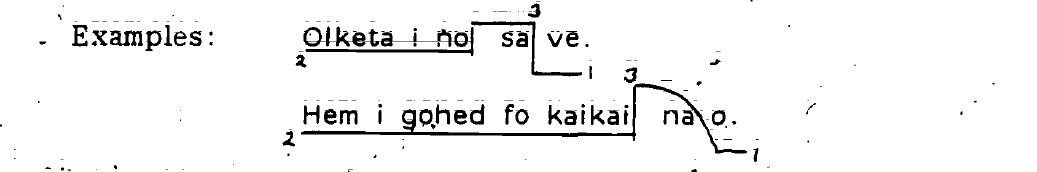
\includegraphics[width=11cm]{intonation.png}
      \caption{\footnotesize{\cite[10]{eric}}}
    \end{figure}
  \end{quote}}
\end{itemize}
\subparagraph{英語との相違点}
\paragraph{関係節標識として} 関係節標識としての使用は無いか、非常に稀である
\begin{itemize}
  \item 英語では制限用法に限って\textit{that}を関係従属節の標識(関係代名詞)として用いることができる\citep[365-367]{english}
  \item Pijin語では通常関係節標識は\textit{we}, \textit{hu} あるいは英語的な文体で稀に\textit{which}が用いられる
  \item この用法はおそらくPijin語にはない: 完全に容認不可能かどうかは確認が必要
\end{itemize}
\paragraph{文中の機能} 直接目的語に限定されている
\begin{itemize}
  \item \cite[1049]{english}ではthat節の文中の機能として5つを挙げている: (a)主語 (b)直接目的語 (c)主格補語 (d)同格 (e)形容詞補語
  \item Pijin語のdat節では用法は(b)しか例が見当たらない
  \item (a)(c)(d)(e)は聖書には出てこない: (a)(c)(d)には\textit{olsem}が、(e)には\textit{fo}が用いられる
  \item 話し言葉でも(a)(c)は\textit{hemi olsem...}の形をよく使うように感じる(cf. (\ref{manguru1})) (d)は単純な挿入が多い
\end{itemize}
\paragraph{olsem} 辞書\citep[157]{dictionary}の説明: 「~のような(like that, as if)」の意味のみ
\begin{comment}
\begin{quote}
  \begin{enumerate}
    \item like, like this, like that; \textbf{Iu bae iu kuki olketa kabis ia olsem ia.} You must cook the vegetables like this.
    \item \textit{sub.} as if; \textbf{Man toktok olsem hem bikman nao.} This man talks as if he were an important man.
  \end{enumerate}
\end{quote}
\end{comment}
\begin{itemize}
  \item 聖書には\textit{olsem}が直接話法を導く標識として登場する(\exn{1})\footnote{義務的ではない。\textit{sei}単独で直接話法を導入する例が多く見つかるが、\textit{sei olsem}の形も184例見つかる}
\end{itemize}
\begin{exe}
  \ex
  \gll Nao olketa \underline{tok} \underline{olsem}, ``Bat bos, hemi garem plande finis ya."\\
  TOP 3PL \underline{say} \underline{like} but boss 3SG-PM have many PERF DIEC\\
  \glt They said, ``But boss, he already have many (money)."(LUK 19:25)
\end{exe}
\begin{itemize}
  \item 聖書では、動詞によって「\textit{olsem}+直接話法」の形を「\textit{dat}+間接話法」の形と使い分けている可能性が高い
  \item 動詞+\textit{olsem} \textit{tok olsem} talk like: 459, \textit{sei olsem} say like: 184, \textit{duim olsem} do like: 75, \textit{stap olsem} be like: 66
  \item 名詞+\textit{olsem} It is that~のような形式主語構文にも用いられるが、本来の推量の意味との区別が難しい \textit{hemi olsem} it is like: 293, \textit{hem olsem} it (is) like: 194, \textit{olketa olsem} they (are) like: 184, \textit{yufala olsem} you(exc.) are like: 64
  \item \textit{talem}のように間接話法で\textit{dat}を取る動詞でも、後ろに直接話法の文が続くと\textit{olsem}が入る
\end{itemize}
\begin{exe}
  \ex
  \gll Buktambu hemi talem klia olsem, ``Bae tufala kamap wanfala bodi nomoa." \\
  book-holy 3SG-PM say clearly like FUT 3DU appear one body only\\
  \glt `The holy book says clearly, ``the two will become one flesh."'(1CO 6:16)
\end{exe}
\begin{itemize}
  \item \textit{dat}の分布とは全く異なる。ただし、これらの数字は従属節標識としてではない形も含んでいる
  \item \textit{dat}とは異なり、形容詞節や副詞節として振る舞っている?さらなる分析が必要
\end{itemize}

\subsection{fo}
\paragraph{従来の意味}
\cite{prepositions} \footnote{(\exn{1}),(\exn{2})はグロス引用, (\exn{3})のグロスは発表者}
\begin{itemize}
  \item 近縁のBislamaやTok Pisinにはない前置詞
  \item 利益者を表す与格的な用法(\exn{1})と目的を示す用法(\exn{2})(\exn{3})がある
  \item 目的を示す場合、後ろに動詞来る: 英語のtoが果たす役割に似ている
\end{itemize}
\begin{exe}
\ex
\gll Mitufala tekem kam samfala sugaken \underline{fo} iu.\\
we.DU.EXC take DIR some sugarcane \underline{DAT} you.SG\\
\glt `We brought you some sugarcane.'
\end{exe}
\begin{exe}
\ex\label{wakalonghem}
\gll An hemi baebae baem samfala tul \underline{fo} waka long hem.\\
and he will buy some tool \underline{to} work LOC it\\
\glt `And he'll buy some tools to work with.'
\end{exe}
\begin{exe}
\ex
\gll Ating iu kam \underline{fo} spoelem mifala ia!\\
probably 2SG come \underline{to} destroy 1PL.EXC DEIC\\
\glt `Probably you've come to destroy us!' (MRK 1:24)
\end{exe}
\paragraph{節を作る前置詞?として}
\begin{itemize}
  \item 聖書には\textit{fo}が主語+動詞を伴って節を作る表現が多く存在する
\end{itemize}
\begin{exe}
\ex\label{setsushugo}
\gll Yu mas tokstrong long olketa fo olketa mas falom.\\
2SG must speak.strongly to 3PL \underline{to} 3PL must follow\\
\glt `You must speak to them strongly enough to follow you.' (1T 6:3)
\ex
\gll Hemi tambu long Lo \underline{fo} yu stap wetem disfala woman ya.\\
3SG-PM prohibitted in Law \underline{for} 2SG be with this woman DEIC\\
\glt `It is prohibitted in Law for you to be with this woman.' (MAT 14:4)
\end{exe}
\subparagraph{調査} (\exn{1}),(\exn{2}) 共に発表者の作った文
\begin{exe}
\ex
\gll Mi laik \underline{fo} yu mekem tok blo yu tru.\\
1SG want \underline{to} 2SG make telling of 2SG true\\
\glt `I want you to talk truth.'
\ex
\gll Hemi tambu \underline{fo} mifala go insaet long disfala ples.\\
3SG-PM prohibitted \underline{to} 1PL.EXC go inside at this place\\
\glt `It is prohibitted for us to enter this place.'
\end{exe}

結果、こちらの文も全て適格であるとみなされた。インフォーマントにこの言い換え表現について尋ねたところ、いずれもこの前置詞句の後置を問題にしたものはなかった一方で、60代のインフォーマント\footnote{脚注5と同一の話者}は次のようなものを提案した。

\begin{exe}
\exi{(\exn{0}$'$)} Hemi tambu \underline{fo} mifala \underline{fo} go insaet long disfala ples.
\end{exe}

(\exn{0})との意味の違いはないが、こちらのほうがより「強い」印象を受けるという。\textit{fo}$+$単語$+$\textit{fo}の組み合わせは聖書コーパス中106件が見つかる。そのうちいくつが主語+前置詞句の組み合わせかは数えていないが、元々2つの前置詞句からなっていた表現が、後ろの前置詞が省略されて節のようになったのかもしれない。ただし、それ以外の話者からこの置き換えが提案されることはなかった\footnote{7人で、Pijin語を母語とする高校生の話者も含む。(\exn{0})も(\exn{0}$'$)も同様に適格な文章であると判断された。}。

\paragraph{英語との相違点}
\begin{itemize}
  \item (\exn{0})では意味的に主語にあたる節の後置が起こっている。これは英語のto不定詞でよく見られる現象である\citep[1062]{english}
  \item しかし、節の主語は英語では別の前置詞句(for)で表される\citep[1061]{english}
  \item 前置詞+主語+動詞の組み合わせは英語では許されない\citep[660]{english}
\end{itemize}
\paragraph{冗長性?}
\begin{itemize}
  \item (\ref{setsushugo})は文の目的語と節主語が, (\ref{bokushi})は文の主語と節主語が同一である
  \item Pijin語では\textit{fo}節で主語が明記されているが、英語に翻訳する際は省略しないと不自然になる
  \item 冗長な文体に思えるが、関係節や前置詞節(cf. (\ref{wakalonghem}))でも冗長に思える代名詞が残るのは事実
  \item ただし、\textit{fo}節の主語は上に比べると省略されることが非常に多いように感じる
\end{itemize}

\section{まとめ・今後の展望}
Pijin語聖書のコーパス分析によって、\textit{dat}, \textit{fo}を従属節標識として頻繁に用いていることが明らかになった。これらはあくまで翻訳された書き言葉であり、本来話し言葉であるPijin語の言語現象と呼ぶには疑念があったが、現地での容認度の調査によって、少なくとも首都ホニアラの話者にとっては、これらの用法がPijin語の枠組みの中で容認されていることが分かった。この調査は10名程度のごく少数の話者への容認度調査であったが、帰国後ラジオの録音等を確認したところ、\textit{dat}, \textit{fo}いずれも従属節標識として用いられている発話例を発見することができた。

ラジオで録音した牧師の演説と思われる発話\footnote{この牧師はソロモン諸島の最近の疾病を聖書の内容と関連付けて演説している。語彙や短い構文で時折英語が混じることはあるが、内容自体は英語からの翻訳ではないと推測できる。}では、\textit{dat}, \textit{fo}いずれも非常によく登場する。長い文章ではあるが、双方が同時に出てくる発話すらある(\exn{1})。

\begin{exe}
\ex\label{bokushi}
\gll Bat taem yu lukim gospel, ... yu mas save dat end hemi kolsap nao fo hemi kam..\\
but when 2SG look gospel ... 2SG must know that end 3SG-PM close TOP for 3SG-PM come\\
\glt `But when you look at the gospel, you must know that the end is coming soon.'
\end{exe}

宗教関連の例文が多いことは気がかりである。実際、1人のインフォーマントは調査の際に、「宗教的な感じがするが、許容できる」といった発言をしていた。特に\textit{dat}については、本来それを使わずにイントネーションで従属節を示す方法があることから、わざわざ使用するのは勿体ぶったような印象を受けるかもしれない。\textit{fo}については、話者がマングローブの管理を語る動画\citep{manguru}にも用例が見つかる\footnote{\textit{is}の導入に見られるように、この話者の発話は英語的な要素が強い(脚注4(iv)と同一の話者である)。しかし、私の意見では、これは少なくとも都市部では一般的な発話である。}。

\begin{exe}
\ex\label{manguru1}
\gll Hem nao olsem main objective nao is fo yumi stadim, documentim all mangrove blo yumi...\\
3SG TOP like main objective TOP (is) for 2SG.PL study document all mangrove POSS 2SG.INC\\
\glt `Main objective for us is to study and document all mangroves that we share.'\citep[20分4秒]{manguru}
\end{exe}

\textit{dat}については、本発表資料の準備を通して動詞目的語の位置にのみ現れ、目的語としての名詞節を作ることしかできないという性質が明らかになってきた。\textit{olsem}や\textit{fo}との使い分けは単純に英語を置き換えただけでは説明できず、さらに分析の余地が残っている。

\textit{fo}については、基本的な分布は英語のto不定詞と同じように感じるが、通常to不定詞では示されない文の主語や目的語と同一の「意味上の主語」が示されることがあるのが興味深い。

今後は可能であれば再度ネイティブスピーカーに協力してもらい、これらの分析について確認をとりたい。また、録音のデータもまだ確認できていない部分がかなり多く残っているので、確認したい。


数百ページにも及ぶ辞書\cite{dictionary}があるにも関わらず、これらの従属節標識についての説明がほとんど無いことの原因として、Pijin語が専ら話し言葉として使われていて、書き言葉としての使用が非常に限定的だということが言えそうである。本論で取り上げた\textit{dat}, \textit{olsem}, \textit{fo}以外にも、話し言葉では頻度が少ないために見過ごされてきた文法事項がまだ残っているように感じられる。
\bibliographystyle{plainnat}
\bibliography{main}

\end{document}
